\documentclass{article}
\usepackage{ifthen}
\usepackage[utf8,utf8x]{inputenc}
\usepackage[a4paper,top=2cm,bottom=2cm,left=2cm,right=2cm]{geometry}
\usepackage[brazil]{babel}
\usepackage{setspace}
\usepackage{graphicx}
\usepackage{url}

% usar para termos estrangeiros
\newcommand{\eng}[1]{\textit{#1}}

% usar para nomes de obras
\newcommand{\opus}[1]{\textit{#1}}

% usar para nomes de termos
\newcommand{\termo}[1]{\textit{#1}}
 
\begin{document}

\setlength{\parindent}{0cm}

%% cabecalho
\large
UNIVERSIDADE FEDERAL DA BAHIA \\
ESCOLA DE MÚSICA \\
PROGRAMA DE PÓS-GRADUAÇÃO \\
MESTRADO EM COMPOSIÇÃO \\
ORIENTADOR: Pedro Kröger \\
ALUNO: Marcos da Silva Sampaio \\
DATA: \today

\thispagestyle{empty}
\vspace{1cm}
\begin{center}
  {\Huge \textbf{Projeto de Dissertação}}
\end{center}
\vspace{1cm}

\section{Introdução}
\label{sec:introducao}

Contorno pode ser definido como o perfil, desenho ou formato de um
objeto. Pode ser bidimensional e associar altura a comprimento,
largura ou tempo. Em música contornos podem ser associados a altura,
densidade, ritmo, complexidade rítmica, homogeneidade orquestral,
amplitude de harmônicos, intensidade, etc. Contornos melódicos estão
relacionados com movimento de altura em função do tempo.
%% Contornos melódicos na composição
Em composição o contorno melódico é um elemento de nível médio de
abstração, entre altura, duração e timbre, e motivos e frases. Sua
presença na música é tão comum quanto a de qualquer outro elemento
citado. 

%% Geração de material composicional

%% "contorno como determinante composicional"
%% falar que assim como tem set, simetria, etc como determinante
%% composicional, contornos podem ser interessantes
Ao estruturar uma obra musical compositores utilizam recursos mais ou
menos abstratos como proporções matemáticas, relações entre alturas
(conjuntos, tonalidades), diversos tipos de simetrias e outros. Tais
recursos já foram bastante analisados e documentados por vários
autores como Lendvai \cite{Lendvai1971}, Howat \cite{Howat1983} e
Babbitt \cite{babbitt1961ssc}. O uso sistemático de contornos
melódicos como determinante composicional também pode ser interessante
na estruturação de uma obra.

%% Teorias de contornos - "sobre contornos"

%%%kroger: o texto está bom, lembre que a citação se refere ao
%%%_artigo_ e não ao autor.

Teorias de contornos têm sido desenvolvidas desde os anos 1980 para
uso em análise musical. Friedmann
\cite{friedmann85:_method_discus_contour,friedmann1987rmc}, Morris
\cite{morris1987cpc}, Marvin e Laprade
\cite{marvin87:_relat_music_contour} e Polansky e Bassein
\cite{polansky92:_possib_impos_melod} iniciaram o desenvolvimento de
teorias de contornos musicais expandindo o trabalho anterior de
etnomusicólogos como Seeger \cite{seeger1960mml}, Kolinski
\cite{kolinkski65:_struc_melod_movem} e Adams
\cite{adams1976mct}.
%% falar da relacao com teoria dos conjuntos (friedmann, morris)
Mais tarde essas teorias foram expandidas por
Quinn \cite{quinn97:_fuzzy_exten_theor_contour}, que se aprofundou na
área de cognição e por Beard \cite{beard2003cmm}, que procurou
descrever matematicamente contornos levando em conta a duração.
%% contorno como determinante composicional:
Clifford \cite{clifford1995cse} e Edworthy \cite{edworthy1985mca}
trataram contornos melódicos como elemento estrutural.

%% TODO: listar exemplos de contornos, e.g. adams
%%       mostrar exemplos de utilização composicional
%%      (tipo: o que temos feito, operações)

Adams \cite{adams1976mct} elaborou uma tipologia de quinze contornos
melódicos reduzindo uma melodia a quatro pontos: primeira e última
notas, nota mais aguda e mais grave. Temos visto a partir de
experiências preliminares de mapeamento desses contornos que entre
alguns deles há relações de inversão e retrogradação. Os contornos
chamados de S1D0 e S3D0, por exemplo guardam entre si uma relação de
retrogradação (ver figura \ref{fig:adams}).

%%% kroger: a frase que começa com "contornos melodicos podem..." está
%%% com problemas na divisão de ideias. as virgulas estão sendo usadas
%%% para separar niveis diferentes. talvez seja bom usar virgulas e
%%% ponto-e-virgulas eu re-rescrever a frase. algumas pessoas podem
%%% argumentar que a partitura é uma representação grafica. talvez
%%% seja bom deixar o "graficamente" mais claro.

Operações como inversão, retrogradação, rotação, transposição,
aumentação e diminuição são musical e matematicamente simples de
implementar. Contornos melódicos podem ser representados musicalmente,
através da partitura; graficamente, a partir de pontos cartesianos
(para melhor entendimento ver figura \ref{fig:adams}); e
simbolicamente com números. Temos feito experiências mapeando essas
operações para contornos melódicos, representando os resultados de
várias maneiras e compondo a partir do uso sistemático de tais
contornos.

%%% kroger: esses exemplos estão muito simples, talvez seja bom ter um
%%% contorno mais detalhado.

\begin{figure}[h]
  \begin{minipage}{1.0\linewidth}
    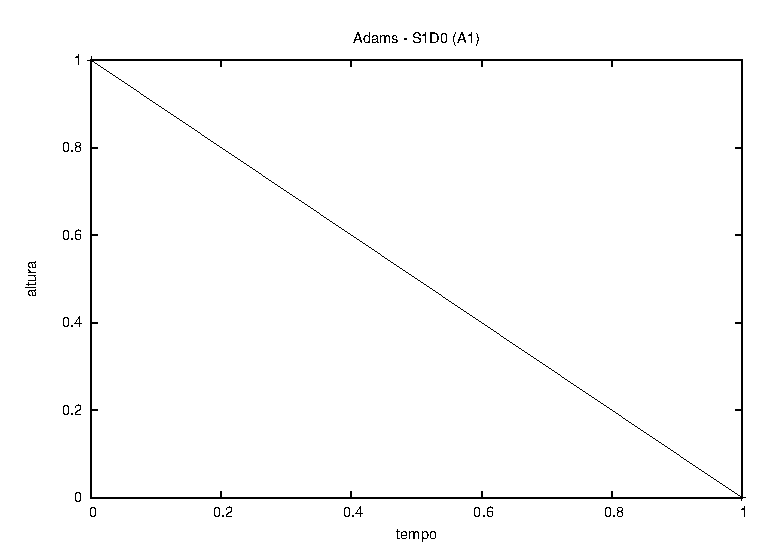
\includegraphics[scale=.6]{a1}
    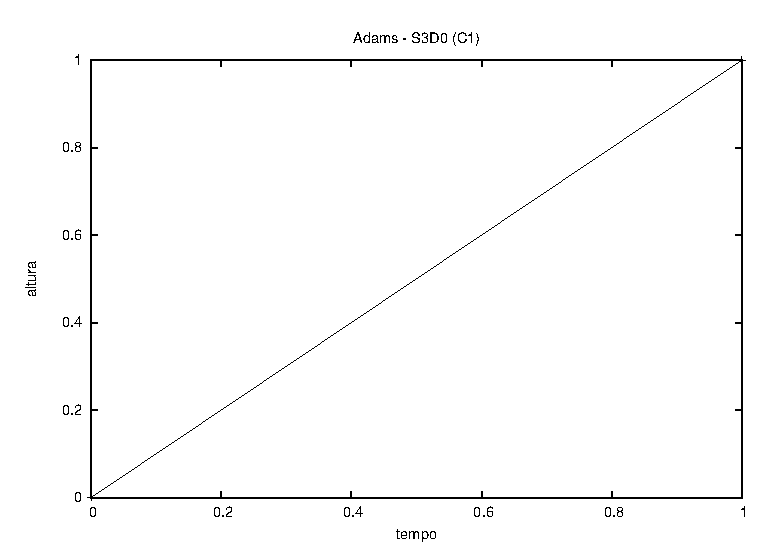
\includegraphics[scale=.6]{c1}
    \centering
  \end{minipage}
  \caption{Contornos de Adams}
  \label{fig:adams}
\end{figure}

%% contornos em análise e em composição

%% enfatizar que terá uma maneira sistematica para trabalhar com
%% contornos

%%% kroger: "estes estudos" não fica claro que são os estudos do
%%% paragrafo antes-do-anterior. fica parecendo que são os estudos do
%%% paragrafo acima. [em geral é uma boa prática escrever cada
%%% paragrafo auto-contido, em geral, "isso", "estes" são palavras
%%% ruins para começar uma frase ou paragrafo porque quebram
%%% \cross{isso} essa ideia de continuidade (viu como o "isso" nessa
%%% frase está ruim? :-)]

As citadas teorias sobre contornos melódicos têm sido desenvolvidos
exclusivamente para análise musical. Nenhum dos trabalhos citados,
entretanto, aborda o uso de contornos melódicos para composição. O uso
sistemático de contornos melódicos pode ser interessante na como
determinante composicional, na estruturação de uma obra musical e na
geração de material composicional.

\section{Objetivos}
\label{sec:objetivos}

O principal objetivo deste projeto é  a composição de uma peça e o seu
memorial.  Esta peça, escrita  para quinteto  de madeiras,  deverá ser
construída com base em material  desenvolvido a partir de operações em
contornos    melódicos   como    transposição,    rotação,   inversão,
retrogradação, aumentação e diminuição, justaposição e superposição.

São objetivos secundários deste trabalho:

%%% kroger: é melhor usar enumeração

\begin{itemize}
\item Desenvolvimento de um programa de computador para processamento
  de operações de contornos melódicos.
\item Entendimento do mapeamento de contornos para elementos
  musicais/composicionais.
\item Compreensão do estado de arte de contornos melódicos.
\end{itemize}

\section{Justificativa}
\label{sec:justificativa}

O uso sistemático de contornos melódicos para geração de material
composicional e como determinante composicional é um assunto carente
de literatura. Seu estudo poderá colaborar com a área de Composição.

\section{Metodologia}
\label{sec:metodologia}

Para a realização deste trabalho deverão ser cumpridas as seguintes
atividades:

\begin{enumerate}
\item Revisão de literatura sobre contornos melódicos

  Para a realização deste trabalho deverá ser feita uma revisão de
  literatura sobre contornos melódicos e assuntos relacionados.

\item Mapeamento de contornos para elementos musicais

  Trata-se da representação de elementos musicais como altura e
  duração para contornos. Envolve o estudo das particularidades de
  tais elementos como representação numérica de notas, intervalos e
  ritmo, bem como estudo de possíveis operações de contornos.

\item Composição de estudos para experimento de possibilidades com
  contornos melódicos.

  Duas peças devem ser compostas para experimentar possibilidades de
  uso de contornos melódicos e operações. A primeira, já concluída,
  contém um único contorno melódico e experimenta possibilidades de
  preenchimento entre os pontos do contorno. A segunda, em andamento,
  testa possibilidades de operações e concatenação. Com esses pequenos
  experimentos é possível aprofundar a prática de composição com
  contornos.

\item Desenvolvimento de um programa de computador para processar
  operações com contornos melódicos.

  Um software que lida com contornos melódicos, operações e
  combinações está sendo desenvolvido. Ele retornará representações
  simbólicas, gráficas e musicais de operações de transposição,
  inversão, retrogradação e rotação de um dado contorno. Além disso
  ele permitirá a combinação de operações e sua concatenação. A
  linguagem é Lisp e a plataforma Unix. Este software ajudará no
  mapeamento e processamento de contornos melódicos tanto no estudo do
  estado de arte, como nos experimentos já realizados com os contornos
  de Adams \cite{adams1976mct}, quanto na composição da obra final.
  
\item Composição da peça

  Todo o material composicional a ser utilizado na peça deverá ser
  gerado por operações e concatenação de operações de contornos
  melódicos, e por preenchimento desses contornos.

\item Escrita da dissertação
\end{enumerate}

\section{Resultados Esperados}
\label{sec:resultados-esperados}

Os resultados pretendidos com este trabalho são a obra para quinteto
de madeiras, o software para processamento de contornos melódicos, o
conhecimento do estado de arte de contornos melódicos e a dissertação
de mestrado, que incluirá a análise da referida obra.

\section{Estrutura de tópicos da dissertação}
\label{sec:estrutura-de-topicos}

\begin{enumerate}
\item Introdução
\item O estado de arte de contornos melódicos
  \begin{enumerate}
  \item Revisão de literatura
  \item Mapeamento de contornos
  \item Ferramentas utilizadas
  \end{enumerate}
\item Análise da composição
\item Partitura da composição
\item Conclusão
\item Bibliografia
\end{enumerate}

\section{Cronograma}
\label{sec:cronograma}

\begin{table}[h]
  \begin{tabular}{lllllllll}
    \hline
    Tarefa & Nov./07 & Dez. & Jan./08 & Fev. & Mar. & Abr. & Mai. \\
    \hline
    Revisão de Literatura & X &  &  & & & & & \\
    Experimentos & X & & & & & & & \\
    Software & X & X & X & X & & & &  \\
    Composição da peça & & X & X & X & X & X \\
    Recital & &  & & & & & X \\
    \hline
  \end{tabular}
\end{table}
\begin{table}[h]
  \begin{tabular}{llllllll}
    \hline
    Tarefa & Jun./08 & Jul. & Ago. & Set. & Out. & Nov. & Dez. \\
    \hline
    Escrita da Dissertação & X & X & X & X & X & & \\
    Entrega da Dissertação & & & & & & X & \\
    Defesa & & & & & & & X \\
    \hline
  \end{tabular}

  \label{tab:cronograma}
\end{table}

\renewcommand{\refname}{Bibliografia}

\nocite{alves05:_invar,buteau2005ama,buteau2003tmm,buteau1999mta,buteau2000csm,cambouropoulos2001mca,cambouropoulos2005pea,clifford1995cse,cook87:_techn_compar_analy,discipio2000ajc,dowling1994mch,dowling1978sac,dowling1971rim,edworthy1985mca,friedmann1987rmc,friedmann85:_method_discus_contour,Hermann1995,hofmannengl1999vpa,ishiyama1996act,kim2000acb,kolinkski65:_struc_melod_movem,lindsay1996ucm,maidin:gam,marvin1988gtm,marvin87:_relat_music_contour,morris93:_new_direc_theor_analy_music_contour,morris1987cpc,parsons1975dta,polansky87mma,polansky92:_possib_impos_melod,quinn2006mcp,quinn97:_fuzzy_exten_theor_contour,ravenscroft2006rcc,music02:_melody,roy2004cbm,schmuckler1999tmm,schubert2006eih,schonberg1967fmc,seeger1960mml,Siu-LanTan04012004,toch1977sfm,toiviainen2002cmm}

\bibliography{mestrado}
\bibliographystyle{plain}

\end{document}